\documentclass[a4paper,11pt,fleqn]{article}%fleqn pour aligner les equations à gauche
\usepackage{../../Styles/Exercice}

\newcommand{\chnum}{Chapitre 16}
\newcommand{\chtitle}{Propagation de la lumière}
\newcommand{\dtype}{Exercices}


\begin{document}
\maketitle
\begin{multicols}{2}
\section{Construire un rayon réfléchi}
Un rayon lumineux provenant d'un laser arriver à la surface d'un bloc de verre représenté en bleu/
\begin{enumerate}
    \item Lire la mesure de l'angle d'incidence.
    \item Déterminer l'angle de réflexion et tracer le rayon réfléchi.
\end{enumerate}
%\begin{figure}[h!]
%    \centering
    \begin{tikzpicture}
%\draw (-3,-3) grid (3,3);
        \draw[fill = yellow!10] (0,0) circle (3);
        \foreach \k in {0,10,...,370}
            \pgfmathsetmacro\xtki{cos(\k)*3 - cos(\k)*0.15}
            \pgfmathsetmacro\xtkj{cos(\k)*3 + cos(\k)*0.15}
            \pgfmathsetmacro\ytki{sin(\k)*3 - sin(\k)*0.15}
            \pgfmathsetmacro\ytkj{sin(\k)*3 + sin(\k)*0.15}            
            \draw (\xtki,\ytki) -- (\xtkj,\ytkj);

    \draw (3,0) node[right]{\SI{0}{\degree}};
    \draw (0,3) node[above]{\SI{90}{\degree}};
    \draw (-3,0) node[left]{\SI{0}{\degree}};
    \draw (0,-3) node[below]{\SI{90}{\degree}};
    \draw[thick,dashed] (-3,0) -- (3,0);
    \draw[thick,dashed] (0,-3) -- (0,3);

    \draw[fill = blue!30!white] (0,-2) rectangle(1.5,2);
    \draw[-Stealth, very thick, red](-3,-3) to (-1,-1);
    \draw[very thick, red](-3,-3) -- (0,0);

    \node (V) at (2.8,2.8){Verre};
    \draw[-stealth,blue] (V) to (1,1);
    \end{tikzpicture}
%    \caption{Caption}
%    \label{fig:enter-label}
%\end{figure}

\section{Calculer un indice de réfraction}
\begin{enumerate}
    \item Identifier les angles d'incidence et de réfraction dans la situation schématisée ci-dessous.
    \item Utiliser la loi de \textsc{snell-descartes} pour calculer l'indice de réfraction de l'eau.
\end{enumerate}

\begin{tikzpicture}
    \fill [green!15] (-5,0) rectangle (3,1.5);
    \fill [blue!15] (-5,-1.5) rectangle (3,0);

    \draw[dashed] (0,-1.5) -- (0,1.5);
    \draw[red] (-5,0) -- (3,0);

    \draw[-Stealth,very thick,red] (-2,1.5) to (-1.6,1.2);
    \draw[very thick,red] (-2,1.5) -- (0,0);

    \draw[-Stealth,very thick,red] (0,0) to (.8,-1.2);
    \draw[very thick,red] (0,0) -- (1,-1.5);
    \draw (0,.25) -- (.25,.25);
    \draw (.25,.25) -- (.25,0);

    \node (Air) at (-4,1){$n_{air}=1,00$};
    \node (Eau) at (-4,-1){$n_{eau}=?$};

    \node (i1) at (-.75,1.25){$i_{1}=\SI{50}{\degree}$};
    \node (i1) at (-.75,-1){$i_{2}=\SI{35}{\degree}$};
    \draw[green!40!black] (0,1)arc(90:142:1);
    \draw[blue!40!black] (0,-1)arc(-90:-55:1);
\end{tikzpicture}

\section{Lumière polychromatique}
Un lumière polychromatique est constituée de trois radiations : bleue, jaune et rouge possédant respectivement les longueurs d'ondes suivantes : $\lambda_{bleu} = \SI{486}{nm}$, $\lambda_{jaune} = \SI{589}{nm}$ et $\lambda_{rouge} = \SI{650}{nm}$.\\
Elle atteint un bloc de verre sous un angle d'incidence $i_1 = \SI{40}{\degree}$ comme indiqué sur le schéma suivant.

\begin{tikzpicture}
    %\fill [green!15] (-5,0) rectangle (3,1.5);
    \fill [blue!15] (-5,-1.5) rectangle (3,0);

    \draw[dashed] (0,-1.5) -- (0,1.5);
    \draw[red] (-5,0) -- (3,0);

    \draw[-Stealth,very thick,red] (-2,1.5) to (-1.6,1.2);
    \draw[very thick,red] (-2,1.5) -- (0,0);
    
    \draw[-Stealth,very thick,blue] (-2.05,1.45) to (-1.65,1.15);
    \draw[very thick,blue] (-2.05,1.45) -- (-.05,-0.05);

    \draw[-Stealth,very thick,yellow] (-1.95,1.55) to (-1.55,1.25);
    \draw[very thick,yellow] (-1.95,1.55) -- (0.05,0.05);

    %\draw[-Stealth,very thick,red] (0,0) to (.8,-1.2);
    %\draw[very thick,red] (0,0) -- (1,-1.5);

    \node (i1) at (-.75,1.25){$i_{1}$};
    \draw[green!40!black] (0,1)arc(90:142:1);
\end{tikzpicture}

\begin{enumerate}
    \item Calculer l'angle de réfraction pour chacune de ces radiations.
    \item Reproduire le schéma puis représenter les trois radiations déviées en respectant leurs positions relatives.
    \item Quelle est la radiation :
    \begin{enumerate}
        \item la plus déviée ?
        \item la moins déviée ?
    \end{enumerate}
    \item Quelle propriété du verre a été mise en évidence ?
\end{enumerate}
\textbf{Données :}
\begin{itemize}
    \item Indice de réfraction du verre pour les différentes radiations : 
    $n_{bleu} =\num{1,516}$ ; $n_{jaune} =\num{1,510}$ ; $n_{rouge} =\num{1,505}$.
    \item Indice de réfraction de l'air : $n_{air} =\num{1,000}$.
\end{itemize}

\section{Réfraction et illusion d'optique}
L'ours, dont la photographie a été prise à travers la paroi d'un bassin aquatique, semble coupé en deux.
\begin{center}
    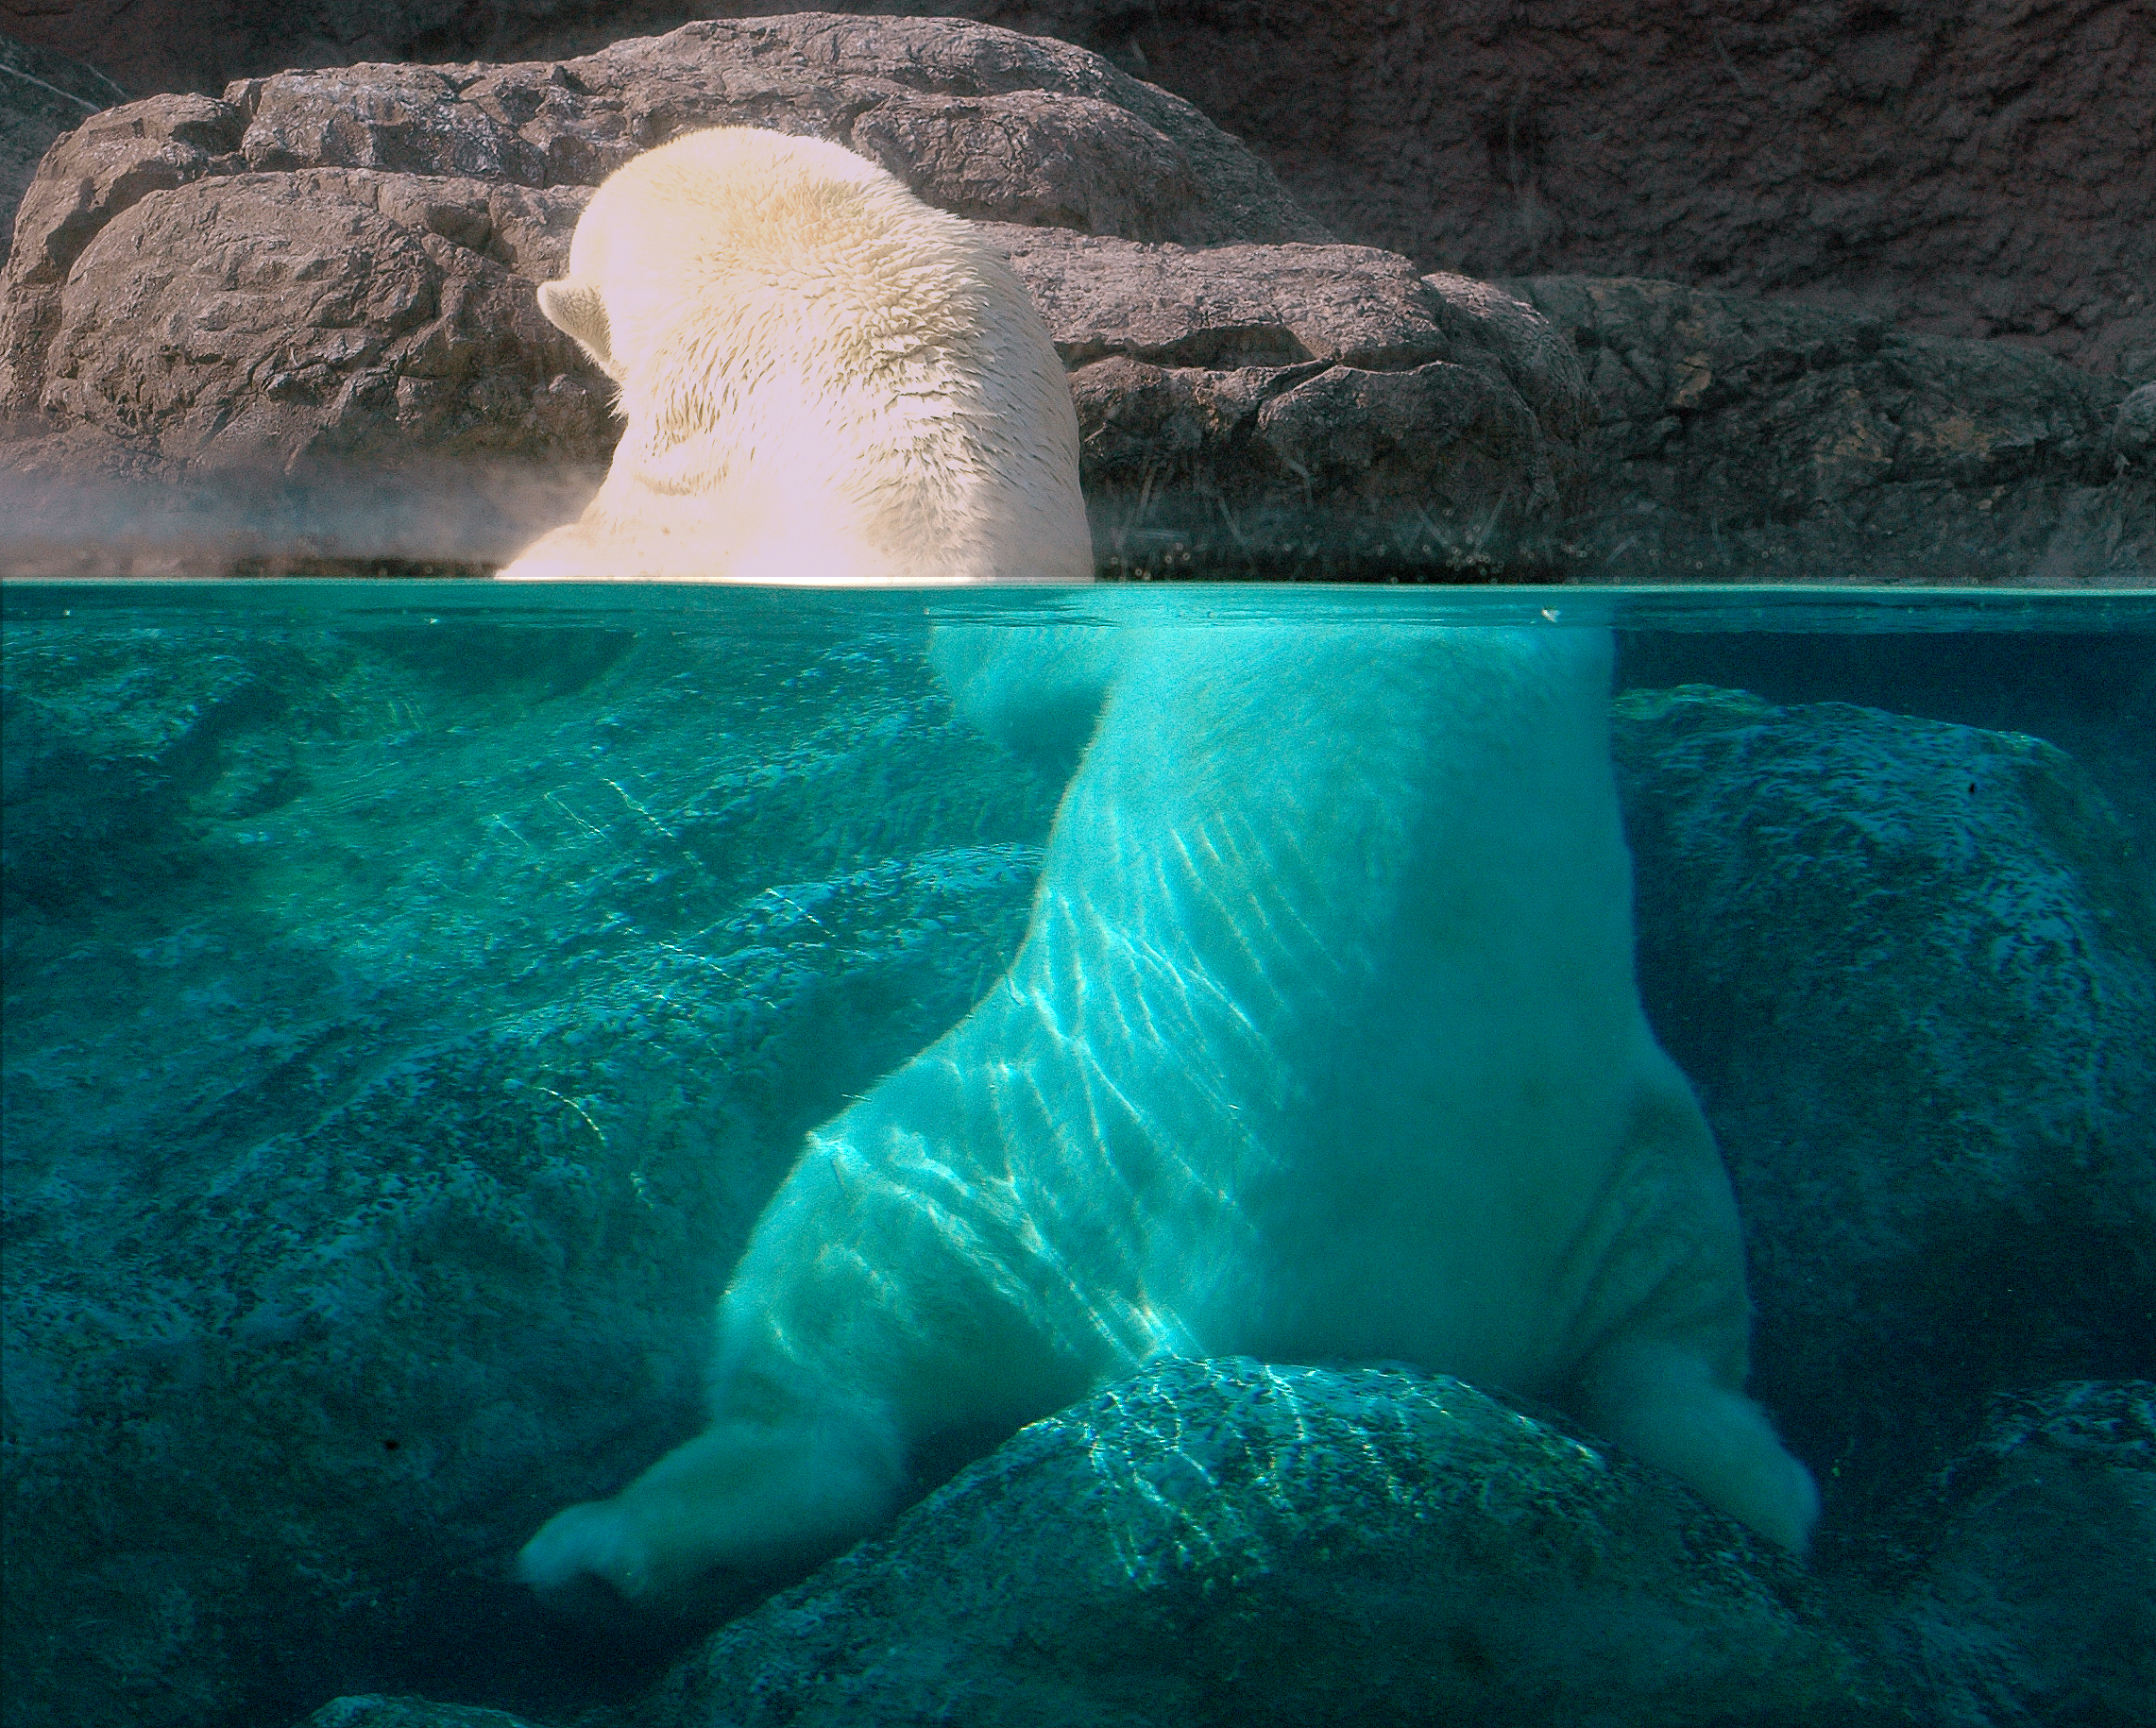
\includegraphics[width=\linewidth]{Ressources/ours_refraction.jpg}
\end{center}
La paroi d'un bassin aquatique est constituée d'une lame de verre à faces parallèles et d'épaisseur \SI{1}{cm}.\\
La lumière diffusée par un point $A$ du corps de l'ours situé au-dessus de l'eau traverse successivement l'air, la paroi de verre avant de se retrouver dans l'air à nouveau. La situation est schématisée ci-dessous.
\begin{center}
    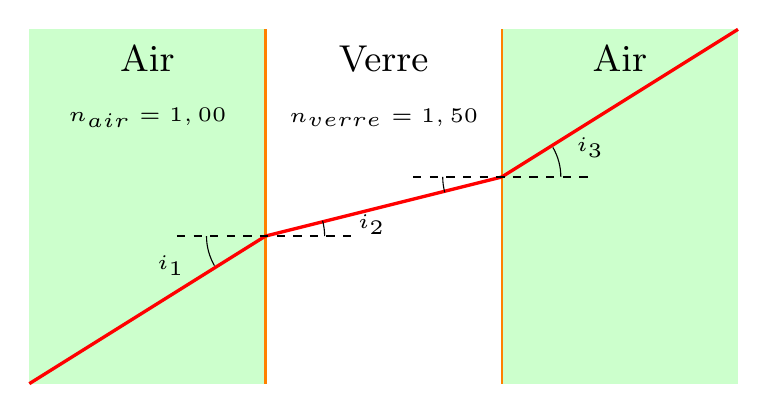
\begin{tikzpicture}[scale=1.5, transform shape]
    \fill[green!20] (0,0) rectangle (2,3);
    \fill[green!20] (4,0) rectangle (6,3);
    \draw[orange,thick] (2,0)--(2,3);
    \draw[orange,thick] (4,0)--(4,3);

    \draw[very thick, red] (0,0) --(2,1.25);
    \draw[very thick, red] (2,1.25) --(4,1.75);
    \draw[very thick, red] (4,1.75) --(6,3);

    \draw[dashed](1.25,1.25) -- (2.75,1.25);

    \draw[dashed](3.25,1.75) -- (4.75,1.75);

    \node (Air1) at (1,2.75){\small Air};
    \node (Verre) at (3,2.75){\small Verre};
    \node (Air2) at (5,2.75){\small Air};

    \node (nair) at (1,2.25){\tiny $n_{air}=1,00$};
    \node (nverre) at (3,2.25){\tiny $n_{verre}=1,50$};

    \draw (1.5,1.25) arc (180:210:.5);
    \draw (2.5,1.25) arc (0:15:.5);

    \draw (3.5,1.75) arc (180:195:.5);
    \draw (4.5,1.75) arc (0:30:.5);

    \node (i1) at (1.2,1){\tiny $i_1$};
    \node (i2) at (2.9,1.35){\tiny $i_2$};
    \node (i3) at (4.75,2){\tiny $i_3$};
\end{tikzpicture}
\end{center}
La lumière diffusée par un point $B$ du corps de l'ours situé au-dessous de l'eau traverse successivement l'eau, la paroi de verre puis l'air. La situation est schématisée ci-dessous.
\begin{center}
    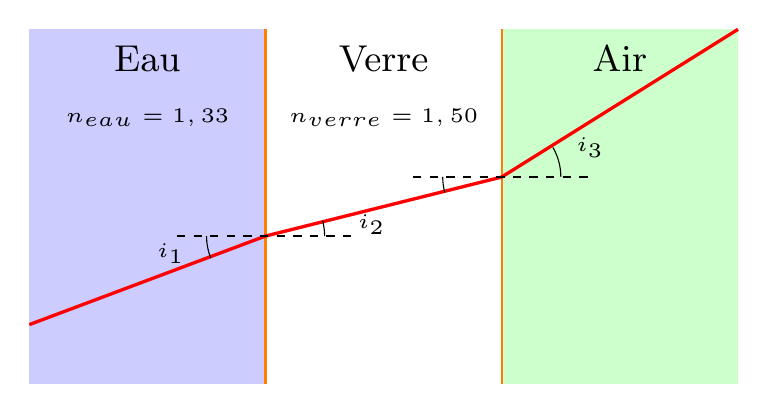
\begin{tikzpicture}[scale=1.5, transform shape]
    \fill[blue!20] (0,0) rectangle (2,3);
    \fill[green!20] (4,0) rectangle (6,3);
    \draw[orange,thick] (2,0)--(2,3);
    \draw[orange,thick] (4,0)--(4,3);

    \draw[very thick, red] (0,.5) --(2,1.25);
    \draw[very thick, red] (2,1.25) --(4,1.75);
    \draw[very thick, red] (4,1.75) --(6,3);

    \draw[dashed](1.25,1.25) -- (2.75,1.25);

    \draw[dashed](3.25,1.75) -- (4.75,1.75);

    \node (Eau) at (1,2.75){\small Eau};
    \node (Verre) at (3,2.75){\small Verre};
    \node (Air2) at (5,2.75){\small Air};

    \node (neau) at (1,2.25){\tiny $n_{eau}=1,33$};
    \node (nverre) at (3,2.25){\tiny $n_{verre}=1,50$};

    \draw (1.5,1.25) arc (180:202:.5);
    \draw (2.5,1.25) arc (0:15:.5);

    \draw (3.5,1.75) arc (180:195:.5);
    \draw (4.5,1.75) arc (0:30:.5);

    \node (i1) at (1.2,1.1){\tiny $i_1$};
    \node (i2) at (2.9,1.35){\tiny $i_2$};
    \node (i3) at (4.75,2){\tiny $i_3$};
\end{tikzpicture}
\end{center}

\begin{enumerate}
    \item Un rayon incident arrive sur la paroi avec un angle d'incidence de \SI{35}{\degree}. Calculer l'angle de réfraction $i_2$ :
    \begin{enumerate}
        \item dans la première situation (point $A$).
        \item dans la deuxième situation (point $B$).
    \end{enumerate}
    \item Pourquoi peut-on écrire que l'on retrouve l'angle $i_2$ en entrée et en sortie de la plaque de verre ?
    \item Calculer l'angle de réfraction $i_3$ du rayon lumineux parvenant à l'observateur :
    \begin{enumerate}
        \item dans la première situation (point $A$).
        \item dans la deuxième situation (point $B$).
    \end{enumerate}
    \item A partir des résultats précédents, expliquer pourquoi l'ours semble coupé en deux sur la photographie.
\end{enumerate}
\end{multicols}
\end{document}